\documentclass[]{article}
\usepackage{lmodern}
\usepackage{amssymb,amsmath}
\usepackage{ifxetex,ifluatex}
\usepackage{fixltx2e} % provides \textsubscript
\ifnum 0\ifxetex 1\fi\ifluatex 1\fi=0 % if pdftex
  \usepackage[T1]{fontenc}
  \usepackage[utf8]{inputenc}
\else % if luatex or xelatex
  \ifxetex
    \usepackage{mathspec}
  \else
    \usepackage{fontspec}
  \fi
  \defaultfontfeatures{Ligatures=TeX,Scale=MatchLowercase}
\fi
% use upquote if available, for straight quotes in verbatim environments
\IfFileExists{upquote.sty}{\usepackage{upquote}}{}
% use microtype if available
\IfFileExists{microtype.sty}{%
\usepackage{microtype}
\UseMicrotypeSet[protrusion]{basicmath} % disable protrusion for tt fonts
}{}
\usepackage[margin=1in]{geometry}
\usepackage{hyperref}
\PassOptionsToPackage{usenames,dvipsnames}{color} % color is loaded by hyperref
\hypersetup{unicode=true,
            pdftitle={Lab 01},
            colorlinks=true,
            linkcolor=Maroon,
            citecolor=Blue,
            urlcolor=Blue,
            breaklinks=true}
\urlstyle{same}  % don't use monospace font for urls
\usepackage{color}
\usepackage{fancyvrb}
\newcommand{\VerbBar}{|}
\newcommand{\VERB}{\Verb[commandchars=\\\{\}]}
\DefineVerbatimEnvironment{Highlighting}{Verbatim}{commandchars=\\\{\}}
% Add ',fontsize=\small' for more characters per line
\usepackage{framed}
\definecolor{shadecolor}{RGB}{248,248,248}
\newenvironment{Shaded}{\begin{snugshade}}{\end{snugshade}}
\newcommand{\AlertTok}[1]{\textcolor[rgb]{0.94,0.16,0.16}{#1}}
\newcommand{\AnnotationTok}[1]{\textcolor[rgb]{0.56,0.35,0.01}{\textbf{\textit{#1}}}}
\newcommand{\AttributeTok}[1]{\textcolor[rgb]{0.13,0.29,0.53}{#1}}
\newcommand{\BaseNTok}[1]{\textcolor[rgb]{0.00,0.00,0.81}{#1}}
\newcommand{\BuiltInTok}[1]{#1}
\newcommand{\CharTok}[1]{\textcolor[rgb]{0.31,0.60,0.02}{#1}}
\newcommand{\CommentTok}[1]{\textcolor[rgb]{0.56,0.35,0.01}{\textit{#1}}}
\newcommand{\CommentVarTok}[1]{\textcolor[rgb]{0.56,0.35,0.01}{\textbf{\textit{#1}}}}
\newcommand{\ConstantTok}[1]{\textcolor[rgb]{0.56,0.35,0.01}{#1}}
\newcommand{\ControlFlowTok}[1]{\textcolor[rgb]{0.13,0.29,0.53}{\textbf{#1}}}
\newcommand{\DataTypeTok}[1]{\textcolor[rgb]{0.13,0.29,0.53}{#1}}
\newcommand{\DecValTok}[1]{\textcolor[rgb]{0.00,0.00,0.81}{#1}}
\newcommand{\DocumentationTok}[1]{\textcolor[rgb]{0.56,0.35,0.01}{\textbf{\textit{#1}}}}
\newcommand{\ErrorTok}[1]{\textcolor[rgb]{0.64,0.00,0.00}{\textbf{#1}}}
\newcommand{\ExtensionTok}[1]{#1}
\newcommand{\FloatTok}[1]{\textcolor[rgb]{0.00,0.00,0.81}{#1}}
\newcommand{\FunctionTok}[1]{\textcolor[rgb]{0.13,0.29,0.53}{\textbf{#1}}}
\newcommand{\ImportTok}[1]{#1}
\newcommand{\InformationTok}[1]{\textcolor[rgb]{0.56,0.35,0.01}{\textbf{\textit{#1}}}}
\newcommand{\KeywordTok}[1]{\textcolor[rgb]{0.13,0.29,0.53}{\textbf{#1}}}
\newcommand{\NormalTok}[1]{#1}
\newcommand{\OperatorTok}[1]{\textcolor[rgb]{0.81,0.36,0.00}{\textbf{#1}}}
\newcommand{\OtherTok}[1]{\textcolor[rgb]{0.56,0.35,0.01}{#1}}
\newcommand{\PreprocessorTok}[1]{\textcolor[rgb]{0.56,0.35,0.01}{\textit{#1}}}
\newcommand{\RegionMarkerTok}[1]{#1}
\newcommand{\SpecialCharTok}[1]{\textcolor[rgb]{0.81,0.36,0.00}{\textbf{#1}}}
\newcommand{\SpecialStringTok}[1]{\textcolor[rgb]{0.31,0.60,0.02}{#1}}
\newcommand{\StringTok}[1]{\textcolor[rgb]{0.31,0.60,0.02}{#1}}
\newcommand{\VariableTok}[1]{\textcolor[rgb]{0.00,0.00,0.00}{#1}}
\newcommand{\VerbatimStringTok}[1]{\textcolor[rgb]{0.31,0.60,0.02}{#1}}
\newcommand{\WarningTok}[1]{\textcolor[rgb]{0.56,0.35,0.01}{\textbf{\textit{#1}}}}
\usepackage{graphicx,grffile}
\makeatletter
\def\maxwidth{\ifdim\Gin@nat@width>\linewidth\linewidth\else\Gin@nat@width\fi}
\def\maxheight{\ifdim\Gin@nat@height>\textheight\textheight\else\Gin@nat@height\fi}
\makeatother
% Scale images if necessary, so that they will not overflow the page
% margins by default, and it is still possible to overwrite the defaults
% using explicit options in \includegraphics[width, height, ...]{}
\setkeys{Gin}{width=\maxwidth,height=\maxheight,keepaspectratio}
\IfFileExists{parskip.sty}{%
\usepackage{parskip}
}{% else
\setlength{\parindent}{0pt}
\setlength{\parskip}{6pt plus 2pt minus 1pt}
}
\setlength{\emergencystretch}{3em}  % prevent overfull lines
\providecommand{\tightlist}{%
  \setlength{\itemsep}{0pt}\setlength{\parskip}{0pt}}
\setcounter{secnumdepth}{0}
% Redefines (sub)paragraphs to behave more like sections
\ifx\paragraph\undefined\else
\let\oldparagraph\paragraph
\renewcommand{\paragraph}[1]{\oldparagraph{#1}\mbox{}}
\fi
\ifx\subparagraph\undefined\else
\let\oldsubparagraph\subparagraph
\renewcommand{\subparagraph}[1]{\oldsubparagraph{#1}\mbox{}}
\fi

%%% Use protect on footnotes to avoid problems with footnotes in titles
\let\rmarkdownfootnote\footnote%
\def\footnote{\protect\rmarkdownfootnote}


  \title{Lab 01}
    \author{}
    \date{}
  

% change section title styling
\usepackage{sectsty}
\sectionfont{\normalsize\normalfont\itshape}
\subsectionfont{\normalsize\normalfont}

% use fancyhdr style
\usepackage{fancyhdr}
\pagestyle{fancy}
\fancyhead[LO, LE]{Lab 01}
\fancyhead[RO, RE]{Env Analysis in R}
\makeatletter
\renewcommand{\maketitle}{\bgroup\vspace*{-1cm}\setlength{\parindent}{0pt}
\begin{flushleft}
  \@author
  
  \@date
  
\end{flushleft}\egroup
}
\makeatother

\begin{document}
\maketitle

\section{Lab 01: An introduction to attribute and spatial analysis in
R}\label{lab-01-an-introduction-to-attribute-and-spatial-analysis-in-r}

\subsubsection{Read the instructions COMPLETELY before starting the
lab}\label{read-the-instructions-completely-before-starting-the-lab}

This lab builds on many of the discussions and exercises from class.
This lab also builds on Chapters 1-3 from your textbook, as well at R
for Data Science by Hadley Wickham and Garrett Grolemund
(\url{https://r4ds.had.co.nz})

\subsubsection{Formatting your
submission}\label{formatting-your-submission}

This lab must be placed into a public repository on GitHub
(www.github.com). Before the due date, submit \textbf{on Canvas} a link
to the repository. I will then download your repositories and run your
code. The code must be contained in either a .R script or a .Rmd
markdown document. As I need to run your code, any data you use in the
lab must be referenced using \textbf{relative path names}. Finally,
answers to questions I pose in this document must also be in the
repository at the time you submit your link to Canvas. They can be in a
separte text file, or if you decide to use an RMarkdown document, you
can answer them directly in the doc.

\subsection{Exploratory data analysis}\label{exploratory-data-analysis}

This lab uses two files from the /data/CBW directory of this course's
main repository: 1. County\_Boundaries.shp: A polygon file containing
the boundaries for all counties in the Chesapeake Bay Watershed 2.
Non-Tidal\_Water\_Quality\_Monitoring\_Stations\_in\_the\_Chesapeake\_Bay.shp:
point locations of non-tidal monitoring stations in the Chesapeake Bay
Watershed

\subsubsection{Step 1, load your packages and
data}\label{step-1-load-your-packages-and-data}

\begin{Shaded}
\begin{Highlighting}[]
\FunctionTok{library}\NormalTok{(tidyverse)}
\end{Highlighting}
\end{Shaded}

\begin{verbatim}
## -- Attaching core tidyverse packages ------------------------ tidyverse 2.0.0 --
## v dplyr     1.1.4     v readr     2.1.5
## v forcats   1.0.0     v stringr   1.5.1
## v ggplot2   3.5.1     v tibble    3.2.1
## v lubridate 1.9.3     v tidyr     1.3.1
## v purrr     1.0.2     
## -- Conflicts ------------------------------------------ tidyverse_conflicts() --
## x dplyr::filter() masks stats::filter()
## x dplyr::lag()    masks stats::lag()
## i Use the conflicted package (<http://conflicted.r-lib.org/>) to force all conflicts to become errors
\end{verbatim}

\begin{Shaded}
\begin{Highlighting}[]
\FunctionTok{library}\NormalTok{(ggplot2) }\CommentTok{\#technically included in tidyverse}
\FunctionTok{library}\NormalTok{(sf)}
\end{Highlighting}
\end{Shaded}

\begin{verbatim}
## Linking to GEOS 3.11.0, GDAL 3.5.3, PROJ 9.1.0; sf_use_s2() is TRUE
\end{verbatim}

\begin{Shaded}
\begin{Highlighting}[]
\FunctionTok{library}\NormalTok{(sp) }\CommentTok{\#just in case}
\end{Highlighting}
\end{Shaded}

Next, load your data:

\begin{Shaded}
\begin{Highlighting}[]
\DocumentationTok{\#\# note the ".." as opposed to "." \textless{}{-} need to go back one additional level from where this file is}
\NormalTok{p.counties }\OtherTok{\textless{}{-}} \StringTok{"../data/CBW/County\_Boundaries.shp"}
\NormalTok{p.stations }\OtherTok{\textless{}{-}} \StringTok{"../data/CBW/Non{-}Tidal\_Water\_Quality\_Monitoring\_Stations\_in\_the\_Chesapeake\_Bay.shp"}


\NormalTok{d.counties }\OtherTok{\textless{}{-}}\NormalTok{ sf}\SpecialCharTok{::}\FunctionTok{read\_sf}\NormalTok{(p.counties)}
\NormalTok{d.stations }\OtherTok{\textless{}{-}}\NormalTok{ sf}\SpecialCharTok{::}\FunctionTok{read\_sf}\NormalTok{(p.stations)}

\FunctionTok{glimpse}\NormalTok{(d.counties)}
\end{Highlighting}
\end{Shaded}

\begin{verbatim}
## Rows: 207
## Columns: 21
## $ OBJECTID   <int> 1, 2, 3, 4, 5, 6, 7, 8, 9, 10, 11, 12, 13, 14, 15, 16, 17, ~
## $ STATEFP10  <chr> "51", "51", "51", "51", "42", "42", "42", "42", "42", "42",~
## $ COUNTYFP10 <chr> "540", "510", "530", "600", "021", "001", "061", "035", "09~
## $ COUNTYNS10 <chr> "01789068", "01498415", "01498417", "01789070", "01213662",~
## $ GEOID10    <chr> "51540", "51510", "51530", "51600", "42021", "42001", "4206~
## $ NAME10     <chr> "Charlottesville", "Alexandria", "Buena Vista", "Fairfax", ~
## $ NAMELSAD10 <chr> "Charlottesville city", "Alexandria city", "Buena Vista cit~
## $ LSAD10     <chr> "25", "25", "25", "25", "06", "06", "06", "06", "06", "06",~
## $ CLASSFP10  <chr> "C7", "C7", "C7", "C7", "H1", "H1", "H1", "H1", "H1", "H1",~
## $ MTFCC10    <chr> "G4020", "G4020", "G4020", "G4020", "G4020", "G4020", "G402~
## $ CSAFP10    <chr> NA, "548", NA, "548", NA, "564", NA, "558", NA, NA, NA, NA,~
## $ CBSAFP10   <chr> "16820", "47900", NA, "47900", "27780", "23900", "26500", "~
## $ METDIVFP10 <chr> NA, "47894", NA, "47894", NA, NA, NA, NA, NA, NA, NA, NA, N~
## $ FUNCSTAT10 <chr> "F", "F", "F", "F", "A", "A", "A", "A", "A", "A", "A", "A",~
## $ ALAND10    <dbl> 26517362, 38919733, 17362236, 16159465, 1782819861, 1343342~
## $ AWATER10   <dbl> 52974, 1140371, 223855, 95054, 13680552, 8081576, 37883358,~
## $ INTPTLAT10 <chr> "+38.0376579", "+38.8183429", "+37.7316634", "+38.8531833",~
## $ INTPTLON10 <chr> "-078.4853806", "-077.0820263", "-079.3563746", "-077.29902~
## $ Shape_Leng <dbl> 47968.96, 43943.77, 34310.52, 29395.95, 260532.87, 195653.0~
## $ Shape_Area <dbl> 42902561, 66086698, 28163001, 26840867, 3109865228, 2297092~
## $ geometry   <MULTIPOLYGON [°]> MULTIPOLYGON (((-78.47071 3..., MULTIPOLYGON (~
\end{verbatim}

\begin{Shaded}
\begin{Highlighting}[]
\FunctionTok{glimpse}\NormalTok{(d.stations)}
\end{Highlighting}
\end{Shaded}

\begin{verbatim}
## Rows: 122
## Columns: 12
## $ OBJECTID   <int> 1, 2, 3, 4, 5, 6, 7, 8, 9, 10, 11, 12, 13, 14, 15, 16, 17, ~
## $ MAP_ID     <int> 1, 2, 3, 4, 5, 6, 7, 8, 9, 10, 11, 12, 13, 14, 15, 16, 17, ~
## $ USGS_STATI <int> 1487000, 1488500, 1491000, 1491500, 1495000, 1502500, 15030~
## $ STATION_NA <chr> "NANTICOKE RIVER NEAR BRIDGEVILLE, DE", "MARSHYHOPE CREEK N~
## $ MAJOR_WATE <chr> "Eastern Shore", "Eastern Shore", "Eastern Shore", "Eastern~
## $ Drainage_A <dbl> 75.39997, 46.79998, 112.99995, 85.19996, 51.59998, 519.9997~
## $ START_DATE <int> 1998, 2005, 1985, 2005, 2005, 2005, 2006, 2005, 2006, 2005,~
## $ END_DATE   <int> 2018, 2018, 2018, 2018, 2018, 2018, 2018, 2018, 2018, 2018,~
## $ Lat        <dbl> 38.72833, 38.84969, 38.99719, 38.96681, 39.66758, 42.37778,~
## $ Long       <dbl> -75.56186, -75.67311, -75.78581, -75.94306, -75.82558, -75.~
## $ STAID      <chr> "01487000", "01488500", "01491000", "01491500", "01495000",~
## $ geometry   <POINT [°]> POINT (-75.56186 38.72834), POINT (-75.67311 38.8497)~
\end{verbatim}

\begin{Shaded}
\begin{Highlighting}[]
\CommentTok{\# check for validity}
\NormalTok{d.stations }\SpecialCharTok{\%\textgreater{}\%}\NormalTok{ sf}\SpecialCharTok{::}\FunctionTok{st\_is\_valid}\NormalTok{()}
\end{Highlighting}
\end{Shaded}

\begin{verbatim}
##   [1] TRUE TRUE TRUE TRUE TRUE TRUE TRUE TRUE TRUE TRUE TRUE TRUE TRUE TRUE TRUE
##  [16] TRUE TRUE TRUE TRUE TRUE TRUE TRUE TRUE TRUE TRUE TRUE TRUE TRUE TRUE TRUE
##  [31] TRUE TRUE TRUE TRUE TRUE TRUE TRUE TRUE TRUE TRUE TRUE TRUE TRUE TRUE TRUE
##  [46] TRUE TRUE TRUE TRUE TRUE TRUE TRUE TRUE TRUE TRUE TRUE TRUE TRUE TRUE TRUE
##  [61] TRUE TRUE TRUE TRUE TRUE TRUE TRUE TRUE TRUE TRUE TRUE TRUE TRUE TRUE TRUE
##  [76] TRUE TRUE TRUE TRUE TRUE TRUE TRUE TRUE TRUE TRUE TRUE TRUE TRUE TRUE TRUE
##  [91] TRUE TRUE TRUE TRUE TRUE TRUE TRUE TRUE TRUE TRUE TRUE TRUE TRUE TRUE TRUE
## [106] TRUE TRUE TRUE TRUE TRUE TRUE TRUE TRUE TRUE TRUE TRUE TRUE TRUE TRUE TRUE
## [121] TRUE TRUE
\end{verbatim}

\begin{Shaded}
\begin{Highlighting}[]
\NormalTok{d.counties }\SpecialCharTok{\%\textgreater{}\%}\NormalTok{ sf}\SpecialCharTok{::}\FunctionTok{st\_is\_valid}\NormalTok{() }\CommentTok{\# returns false for one feature, so we need to fix}
\end{Highlighting}
\end{Shaded}

\begin{verbatim}
##   [1]  TRUE  TRUE  TRUE  TRUE  TRUE  TRUE  TRUE  TRUE  TRUE  TRUE  TRUE  TRUE
##  [13]  TRUE  TRUE  TRUE  TRUE  TRUE  TRUE  TRUE  TRUE  TRUE  TRUE  TRUE  TRUE
##  [25]  TRUE  TRUE  TRUE  TRUE  TRUE  TRUE  TRUE  TRUE  TRUE  TRUE  TRUE  TRUE
##  [37]  TRUE  TRUE  TRUE  TRUE  TRUE  TRUE  TRUE  TRUE  TRUE  TRUE  TRUE  TRUE
##  [49]  TRUE  TRUE  TRUE  TRUE  TRUE  TRUE  TRUE  TRUE  TRUE  TRUE  TRUE  TRUE
##  [61]  TRUE  TRUE  TRUE  TRUE  TRUE  TRUE  TRUE  TRUE  TRUE  TRUE  TRUE  TRUE
##  [73]  TRUE  TRUE  TRUE  TRUE  TRUE  TRUE  TRUE  TRUE  TRUE  TRUE  TRUE  TRUE
##  [85]  TRUE  TRUE  TRUE  TRUE  TRUE  TRUE  TRUE  TRUE  TRUE  TRUE  TRUE  TRUE
##  [97]  TRUE  TRUE  TRUE  TRUE  TRUE  TRUE  TRUE  TRUE  TRUE  TRUE  TRUE  TRUE
## [109]  TRUE  TRUE  TRUE  TRUE  TRUE  TRUE  TRUE  TRUE  TRUE  TRUE  TRUE  TRUE
## [121]  TRUE  TRUE  TRUE  TRUE  TRUE  TRUE  TRUE  TRUE  TRUE  TRUE  TRUE  TRUE
## [133]  TRUE  TRUE  TRUE  TRUE  TRUE  TRUE  TRUE  TRUE  TRUE  TRUE  TRUE  TRUE
## [145]  TRUE  TRUE  TRUE  TRUE  TRUE  TRUE  TRUE  TRUE  TRUE  TRUE  TRUE  TRUE
## [157]  TRUE  TRUE  TRUE  TRUE  TRUE  TRUE  TRUE  TRUE  TRUE  TRUE  TRUE  TRUE
## [169]  TRUE  TRUE  TRUE  TRUE  TRUE  TRUE  TRUE  TRUE  TRUE  TRUE  TRUE  TRUE
## [181]  TRUE  TRUE  TRUE  TRUE  TRUE  TRUE  TRUE  TRUE  TRUE  TRUE  TRUE  TRUE
## [193]  TRUE  TRUE  TRUE  TRUE  TRUE  TRUE  TRUE  TRUE  TRUE  TRUE  TRUE  TRUE
## [205]  TRUE FALSE  TRUE
\end{verbatim}

\begin{Shaded}
\begin{Highlighting}[]
\CommentTok{\# fix it "in place"}
\NormalTok{d.counties }\OtherTok{\textless{}{-}}\NormalTok{ d.counties }\SpecialCharTok{\%\textgreater{}\%}\NormalTok{ sf}\SpecialCharTok{::}\FunctionTok{st\_make\_valid}\NormalTok{()}
\end{Highlighting}
\end{Shaded}

In class, we discussed how to use dplyr verbs such as \emph{filter},
\emph{select}, and \emph{mutate}. There are some useful cheatsheets on
the RStudio website to help with \emph{dplyr}, \emph{ggplot}, and other
functions here: \url{https://www.rstudio.com/resources/cheatsheets/}

Let's start with the \emph{select} function, which SELECTS attributes
that we specify:

\begin{Shaded}
\begin{Highlighting}[]
\NormalTok{d.counties }\SpecialCharTok{\%\textgreater{}\%}\NormalTok{ dplyr}\SpecialCharTok{::}\FunctionTok{select}\NormalTok{(GEOID10, ALAND10) }\SpecialCharTok{\%\textgreater{}\%} \FunctionTok{head}\NormalTok{()}
\end{Highlighting}
\end{Shaded}

\begin{verbatim}
## Simple feature collection with 6 features and 2 fields
## Geometry type: MULTIPOLYGON
## Dimension:     XY
## Bounding box:  xmin: -79.38264 ymin: 37.69574 xmax: -76.95493 ymax: 40.72605
## Geodetic CRS:  WGS 84
## # A tibble: 6 x 3
##   GEOID10    ALAND10                                                    geometry
##   <chr>        <dbl>                                          <MULTIPOLYGON [°]>
## 1 51540     26517362 (((-78.47082 38.04893, -78.47086 38.04893, -78.47096 38.04~
## 2 51510     38919733 (((-77.06129 38.79457, -77.0612 38.79454, -77.06092 38.794~
## 3 51530     17362236 (((-79.36668 37.7267, -79.36655 37.72627, -79.36653 37.726~
## 4 51600     16159465 (((-77.31476 38.86701, -77.31534 38.86702, -77.31537 38.86~
## 5 42021   1782819861 (((-79.03546 40.31539, -79.03611 40.31477, -79.0363 40.314~
## 6 42001   1343342705 (((-77.46594 39.85958, -77.46589 39.85924, -77.46586 39.85~
\end{verbatim}

\begin{Shaded}
\begin{Highlighting}[]
\CommentTok{\# head truncates the data.frame to the first n rows}
\end{Highlighting}
\end{Shaded}

Note that because we're using a spatial data frame in the \texttt{sf}
package, the geometry is preserved, even though we didn't specify it. We
can also get rid of attributes we DON'T WANT (but not the geometry
attribute) using a \texttt{-} flag. For example:

\begin{Shaded}
\begin{Highlighting}[]
\NormalTok{d.counties }\SpecialCharTok{\%\textgreater{}\%}\NormalTok{ dplyr}\SpecialCharTok{::}\FunctionTok{select}\NormalTok{(}\SpecialCharTok{{-}}\NormalTok{NAME10) }\SpecialCharTok{\%\textgreater{}\%} \FunctionTok{head}\NormalTok{()}
\end{Highlighting}
\end{Shaded}

\begin{verbatim}
## Simple feature collection with 6 features and 19 fields
## Geometry type: MULTIPOLYGON
## Dimension:     XY
## Bounding box:  xmin: -79.38264 ymin: 37.69574 xmax: -76.95493 ymax: 40.72605
## Geodetic CRS:  WGS 84
## # A tibble: 6 x 20
##   OBJECTID STATEFP10 COUNTYFP10 COUNTYNS10 GEOID10 NAMELSAD10   LSAD10 CLASSFP10
##      <int> <chr>     <chr>      <chr>      <chr>   <chr>        <chr>  <chr>    
## 1        1 51        540        01789068   51540   Charlottesv~ 25     C7       
## 2        2 51        510        01498415   51510   Alexandria ~ 25     C7       
## 3        3 51        530        01498417   51530   Buena Vista~ 25     C7       
## 4        4 51        600        01789070   51600   Fairfax city 25     C7       
## 5        5 42        021        01213662   42021   Cambria Cou~ 06     H1       
## 6        6 42        001        01213656   42001   Adams County 06     H1       
## # i 12 more variables: MTFCC10 <chr>, CSAFP10 <chr>, CBSAFP10 <chr>,
## #   METDIVFP10 <chr>, FUNCSTAT10 <chr>, ALAND10 <dbl>, AWATER10 <dbl>,
## #   INTPTLAT10 <chr>, INTPTLON10 <chr>, Shape_Leng <dbl>, Shape_Area <dbl>,
## #   geometry <MULTIPOLYGON [°]>
\end{verbatim}

We can also specify ranges that we want to keep (or not):

\begin{Shaded}
\begin{Highlighting}[]
\NormalTok{d.counties }\SpecialCharTok{\%\textgreater{}\%}\NormalTok{ dplyr}\SpecialCharTok{::}\FunctionTok{select}\NormalTok{(GEOID10}\SpecialCharTok{:}\NormalTok{CLASSFP10) }\SpecialCharTok{\%\textgreater{}\%} \FunctionTok{head}\NormalTok{() }
\end{Highlighting}
\end{Shaded}

\begin{verbatim}
## Simple feature collection with 6 features and 5 fields
## Geometry type: MULTIPOLYGON
## Dimension:     XY
## Bounding box:  xmin: -79.38264 ymin: 37.69574 xmax: -76.95493 ymax: 40.72605
## Geodetic CRS:  WGS 84
## # A tibble: 6 x 6
##   GEOID10 NAME10          NAMELSAD10  LSAD10 CLASSFP10                  geometry
##   <chr>   <chr>           <chr>       <chr>  <chr>            <MULTIPOLYGON [°]>
## 1 51540   Charlottesville Charlottes~ 25     C7        (((-78.47082 38.04893, -~
## 2 51510   Alexandria      Alexandria~ 25     C7        (((-77.06129 38.79457, -~
## 3 51530   Buena Vista     Buena Vist~ 25     C7        (((-79.36668 37.7267, -7~
## 4 51600   Fairfax         Fairfax ci~ 25     C7        (((-77.31476 38.86701, -~
## 5 42021   Cambria         Cambria Co~ 06     H1        (((-79.03546 40.31539, -~
## 6 42001   Adams           Adams Coun~ 06     H1        (((-77.46594 39.85958, -~
\end{verbatim}

\begin{Shaded}
\begin{Highlighting}[]
\NormalTok{d.counties }\SpecialCharTok{\%\textgreater{}\%}\NormalTok{ dplyr}\SpecialCharTok{::}\FunctionTok{select}\NormalTok{(}\SpecialCharTok{{-}}\NormalTok{(GEOID10}\SpecialCharTok{:}\NormalTok{CLASSFP10)) }\SpecialCharTok{\%\textgreater{}\%} \FunctionTok{head}\NormalTok{() }
\end{Highlighting}
\end{Shaded}

\begin{verbatim}
## Simple feature collection with 6 features and 15 fields
## Geometry type: MULTIPOLYGON
## Dimension:     XY
## Bounding box:  xmin: -79.38264 ymin: 37.69574 xmax: -76.95493 ymax: 40.72605
## Geodetic CRS:  WGS 84
## # A tibble: 6 x 16
##   OBJECTID STATEFP10 COUNTYFP10 COUNTYNS10 MTFCC10 CSAFP10 CBSAFP10 METDIVFP10
##      <int> <chr>     <chr>      <chr>      <chr>   <chr>   <chr>    <chr>     
## 1        1 51        540        01789068   G4020   <NA>    16820    <NA>      
## 2        2 51        510        01498415   G4020   548     47900    47894     
## 3        3 51        530        01498417   G4020   <NA>    <NA>     <NA>      
## 4        4 51        600        01789070   G4020   548     47900    47894     
## 5        5 42        021        01213662   G4020   <NA>    27780    <NA>      
## 6        6 42        001        01213656   G4020   564     23900    <NA>      
## # i 8 more variables: FUNCSTAT10 <chr>, ALAND10 <dbl>, AWATER10 <dbl>,
## #   INTPTLAT10 <chr>, INTPTLON10 <chr>, Shape_Leng <dbl>, Shape_Area <dbl>,
## #   geometry <MULTIPOLYGON [°]>
\end{verbatim}

\begin{Shaded}
\begin{Highlighting}[]
\NormalTok{d.counties }\SpecialCharTok{\%\textgreater{}\%}\NormalTok{ dplyr}\SpecialCharTok{::}\FunctionTok{select}\NormalTok{(}\FunctionTok{starts\_with}\NormalTok{(}\StringTok{"C"}\NormalTok{))}
\end{Highlighting}
\end{Shaded}

\begin{verbatim}
## Simple feature collection with 207 features and 5 fields
## Geometry type: MULTIPOLYGON
## Dimension:     XY
## Bounding box:  xmin: -81.01449 ymin: 36.55035 xmax: -74.16468 ymax: 44.09697
## Geodetic CRS:  WGS 84
## # A tibble: 207 x 6
##    COUNTYFP10 COUNTYNS10 CLASSFP10 CSAFP10 CBSAFP10                     geometry
##    <chr>      <chr>      <chr>     <chr>   <chr>              <MULTIPOLYGON [°]>
##  1 540        01789068   C7        <NA>    16820    (((-78.47082 38.04893, -78.~
##  2 510        01498415   C7        548     47900    (((-77.06129 38.79457, -77.~
##  3 530        01498417   C7        <NA>    <NA>     (((-79.36668 37.7267, -79.3~
##  4 600        01789070   C7        548     47900    (((-77.31476 38.86701, -77.~
##  5 021        01213662   H1        <NA>    27780    (((-79.03546 40.31539, -79.~
##  6 001        01213656   H1        564     23900    (((-77.46594 39.85958, -77.~
##  7 061        01213672   H1        <NA>    26500    (((-78.14963 40.1743, -78.1~
##  8 035        01214721   H1        558     30820    (((-78.05375 41.27349, -78.~
##  9 093        01213681   H1        <NA>    14100    (((-76.55799 40.93887, -76.~
## 10 117        01209189   H1        <NA>    <NA>     (((-77.21985 41.99978, -77.~
## # i 197 more rows
\end{verbatim}

\subsubsection{Grouping data}\label{grouping-data}

We can also ``group'' our data according to categorical data in our
data.frames. This is useful if you want to create a function that works
across the entire group. For example, we'll create a new attribute the
calculates the land area of all counties in each state.

\begin{Shaded}
\begin{Highlighting}[]
\NormalTok{d.counties }\SpecialCharTok{\%\textgreater{}\%} \FunctionTok{group\_by}\NormalTok{(STATEFP10) }\SpecialCharTok{\%\textgreater{}\%} \FunctionTok{mutate}\NormalTok{(}\AttributeTok{stateLandArea =} \FunctionTok{sum}\NormalTok{(ALAND10))}
\end{Highlighting}
\end{Shaded}

\begin{verbatim}
## Simple feature collection with 207 features and 21 fields
## Geometry type: MULTIPOLYGON
## Dimension:     XY
## Bounding box:  xmin: -81.01449 ymin: 36.55035 xmax: -74.16468 ymax: 44.09697
## Geodetic CRS:  WGS 84
## # A tibble: 207 x 22
## # Groups:   STATEFP10 [7]
##    OBJECTID STATEFP10 COUNTYFP10 COUNTYNS10 GEOID10 NAME10     NAMELSAD10 LSAD10
##  *    <int> <chr>     <chr>      <chr>      <chr>   <chr>      <chr>      <chr> 
##  1        1 51        540        01789068   51540   Charlotte~ Charlotte~ 25    
##  2        2 51        510        01498415   51510   Alexandria Alexandri~ 25    
##  3        3 51        530        01498417   51530   Buena Vis~ Buena Vis~ 25    
##  4        4 51        600        01789070   51600   Fairfax    Fairfax c~ 25    
##  5        5 42        021        01213662   42021   Cambria    Cambria C~ 06    
##  6        6 42        001        01213656   42001   Adams      Adams Cou~ 06    
##  7        7 42        061        01213672   42061   Huntingdon Huntingdo~ 06    
##  8        8 42        035        01214721   42035   Clinton    Clinton C~ 06    
##  9        9 42        093        01213681   42093   Montour    Montour C~ 06    
## 10       10 42        117        01209189   42117   Tioga      Tioga Cou~ 06    
## # i 197 more rows
## # i 14 more variables: CLASSFP10 <chr>, MTFCC10 <chr>, CSAFP10 <chr>,
## #   CBSAFP10 <chr>, METDIVFP10 <chr>, FUNCSTAT10 <chr>, ALAND10 <dbl>,
## #   AWATER10 <dbl>, INTPTLAT10 <chr>, INTPTLON10 <chr>, Shape_Leng <dbl>,
## #   Shape_Area <dbl>, geometry <MULTIPOLYGON [°]>, stateLandArea <dbl>
\end{verbatim}

The above function is useful if you want to make calculations ``in
place'' and use them in further row-by-row functions. However, we can
further summarize our data such that we don't see all the extra data not
relevant to our query. Note that sometimes buggy geometry can affect
normal dplyr functions, so the code below converts the sf data frame to
a tibble, then removes the geometry before performing the
\texttt{group\_by} and \texttt{summarise} functions. This is an
unnecessary step when using validated geometry, but can also speed up
computation.

\begin{Shaded}
\begin{Highlighting}[]
\NormalTok{d.counties }\SpecialCharTok{\%\textgreater{}\%} 
  \FunctionTok{as\_tibble}\NormalTok{() }\SpecialCharTok{\%\textgreater{}\%}\NormalTok{ dplyr}\SpecialCharTok{::}\FunctionTok{select}\NormalTok{(}\SpecialCharTok{{-}}\NormalTok{geometry) }\SpecialCharTok{\%\textgreater{}\%} \CommentTok{\# this line converts the data because of wonky geometry}
  \FunctionTok{group\_by}\NormalTok{(STATEFP10) }\SpecialCharTok{\%\textgreater{}\%} 
  \FunctionTok{summarise}\NormalTok{(}\AttributeTok{stateLandArea =} \FunctionTok{sum}\NormalTok{(ALAND10))}
\end{Highlighting}
\end{Shaded}

\begin{verbatim}
## # A tibble: 7 x 2
##   STATEFP10 stateLandArea
##   <chr>             <dbl>
## 1 10           5046703785
## 2 11            158114680
## 3 24          25141638381
## 4 36          40599407643
## 5 42          78174288199
## 6 51          69471293533
## 7 54          20781223859
\end{verbatim}

\ldots and we're left with a sum of all the land area in each state (by
FIPS code)

\subsubsection{A diversion into plots}\label{a-diversion-into-plots}

We can also use grouping functions in our visualization. For example:

\begin{Shaded}
\begin{Highlighting}[]
\NormalTok{d.counties }\SpecialCharTok{\%\textgreater{}\%} 
  \FunctionTok{ggplot}\NormalTok{(., }\FunctionTok{aes}\NormalTok{(}\AttributeTok{x =} \FunctionTok{as.factor}\NormalTok{(STATEFP10), }\AttributeTok{y =}\NormalTok{ ALAND10)) }\SpecialCharTok{+}
  \FunctionTok{geom\_boxplot}\NormalTok{(}\FunctionTok{aes}\NormalTok{(}\AttributeTok{fill =}\NormalTok{ STATEFP10))}
\end{Highlighting}
\end{Shaded}

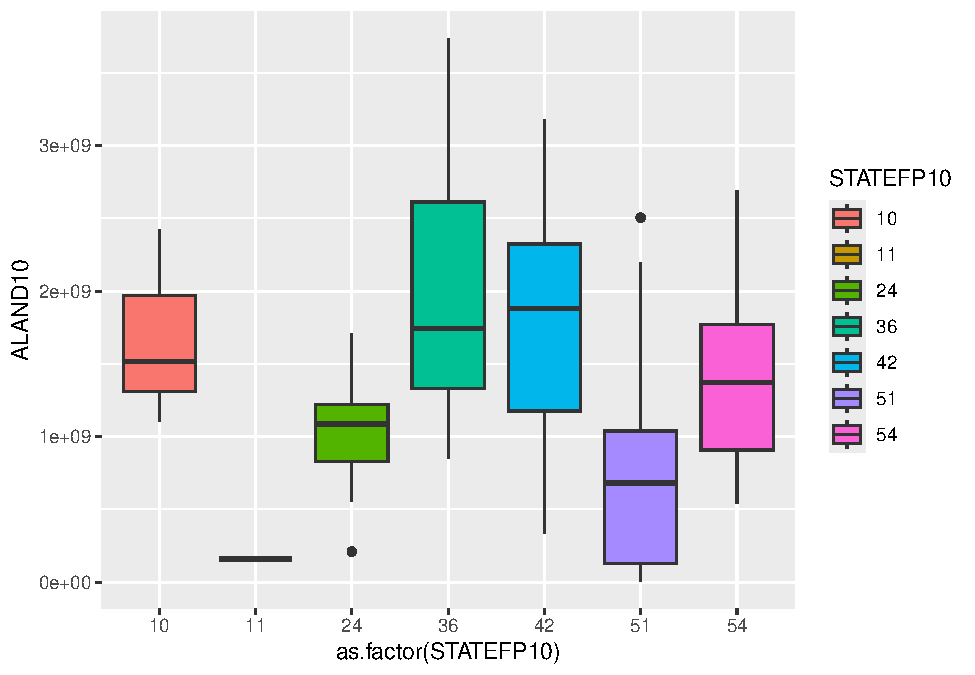
\includegraphics{lab01_files/figure-latex/plots-1.pdf} Or:

\begin{Shaded}
\begin{Highlighting}[]
\NormalTok{d.counties }\SpecialCharTok{\%\textgreater{}\%} 
  \FunctionTok{ggplot}\NormalTok{(., }\FunctionTok{aes}\NormalTok{(}\AttributeTok{x =}\NormalTok{ ALAND10)) }\SpecialCharTok{+}
  \FunctionTok{geom\_histogram}\NormalTok{(}\FunctionTok{aes}\NormalTok{(}\AttributeTok{fill =}\NormalTok{ STATEFP10)) }\SpecialCharTok{+}
  \FunctionTok{labs}\NormalTok{(}\AttributeTok{title =} \StringTok{"not the most useful plot, but you get the idea"}\NormalTok{)}
\end{Highlighting}
\end{Shaded}

\begin{verbatim}
## `stat_bin()` using `bins = 30`. Pick better value with `binwidth`.
\end{verbatim}

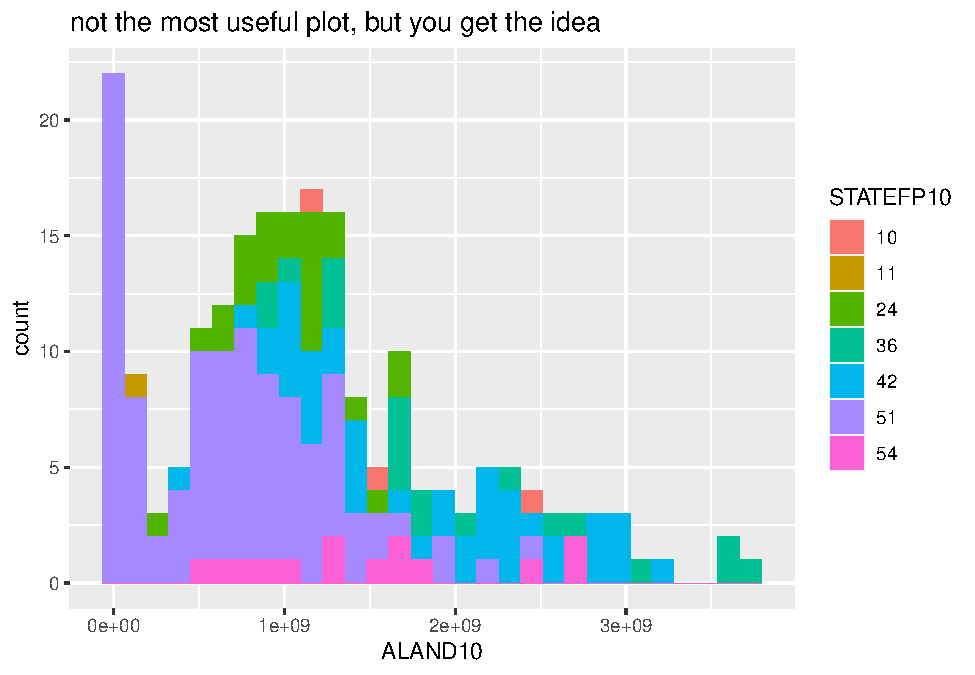
\includegraphics{lab01_files/figure-latex/plots2-1.pdf}

\subsubsection{Spatial operations}\label{spatial-operations}

Since we have spatial data, we can peform some basic spatial operations
with it. First, let's take a look at the coordinate reference system
(CRS) for each file:

\begin{Shaded}
\begin{Highlighting}[]
\NormalTok{d.counties }\SpecialCharTok{\%\textgreater{}\%}\NormalTok{ sf}\SpecialCharTok{::}\FunctionTok{st\_crs}\NormalTok{()}
\end{Highlighting}
\end{Shaded}

\begin{verbatim}
## Coordinate Reference System:
##   User input: WGS 84 
##   wkt:
## GEOGCRS["WGS 84",
##     DATUM["World Geodetic System 1984",
##         ELLIPSOID["WGS 84",6378137,298.257223563,
##             LENGTHUNIT["metre",1]]],
##     PRIMEM["Greenwich",0,
##         ANGLEUNIT["degree",0.0174532925199433]],
##     CS[ellipsoidal,2],
##         AXIS["latitude",north,
##             ORDER[1],
##             ANGLEUNIT["degree",0.0174532925199433]],
##         AXIS["longitude",east,
##             ORDER[2],
##             ANGLEUNIT["degree",0.0174532925199433]],
##     ID["EPSG",4326]]
\end{verbatim}

\begin{Shaded}
\begin{Highlighting}[]
\NormalTok{d.stations }\SpecialCharTok{\%\textgreater{}\%}\NormalTok{ sf}\SpecialCharTok{::}\FunctionTok{st\_crs}\NormalTok{()}
\end{Highlighting}
\end{Shaded}

\begin{verbatim}
## Coordinate Reference System:
##   User input: WGS 84 
##   wkt:
## GEOGCRS["WGS 84",
##     DATUM["World Geodetic System 1984",
##         ELLIPSOID["WGS 84",6378137,298.257223563,
##             LENGTHUNIT["metre",1]]],
##     PRIMEM["Greenwich",0,
##         ANGLEUNIT["degree",0.0174532925199433]],
##     CS[ellipsoidal,2],
##         AXIS["latitude",north,
##             ORDER[1],
##             ANGLEUNIT["degree",0.0174532925199433]],
##         AXIS["longitude",east,
##             ORDER[2],
##             ANGLEUNIT["degree",0.0174532925199433]],
##     ID["EPSG",4326]]
\end{verbatim}

They're the same, but we can formally check

\begin{Shaded}
\begin{Highlighting}[]
\NormalTok{d.counties }\SpecialCharTok{\%\textgreater{}\%}\NormalTok{ sf}\SpecialCharTok{::}\FunctionTok{st\_crs}\NormalTok{() }\SpecialCharTok{==}\NormalTok{ d.stations }\SpecialCharTok{\%\textgreater{}\%}\NormalTok{ sf}\SpecialCharTok{::}\FunctionTok{st\_crs}\NormalTok{()}
\end{Highlighting}
\end{Shaded}

\begin{verbatim}
## [1] TRUE
\end{verbatim}

We need to make sure the files have the same CRS before we do our
spatial operations using the both of them. But to make the problem more
tractable, let's first pare down our data such that we only have the
counties in the state of Delaware:

\begin{Shaded}
\begin{Highlighting}[]
\NormalTok{del.counties }\OtherTok{\textless{}{-}}\NormalTok{ d.counties }\SpecialCharTok{\%\textgreater{}\%}\NormalTok{ dplyr}\SpecialCharTok{::}\FunctionTok{filter}\NormalTok{(STATEFP10 }\SpecialCharTok{==} \DecValTok{10}\NormalTok{)}
\end{Highlighting}
\end{Shaded}

then, we can perform a \emph{spatial intersection} to find all of the
monitoring stations within our Delaware subset

\begin{Shaded}
\begin{Highlighting}[]
\NormalTok{del.stations }\OtherTok{\textless{}{-}}\NormalTok{ sf}\SpecialCharTok{::}\FunctionTok{st\_intersection}\NormalTok{(d.stations, del.counties)}
\end{Highlighting}
\end{Shaded}

\begin{verbatim}
## Warning: attribute variables are assumed to be spatially constant throughout
## all geometries
\end{verbatim}

Plotting this small number of points will be ok, so let's look at the
data first, then check the plot:

\begin{Shaded}
\begin{Highlighting}[]
\FunctionTok{glimpse}\NormalTok{(del.stations)}
\end{Highlighting}
\end{Shaded}

\begin{verbatim}
## Rows: 2
## Columns: 32
## $ OBJECTID   <int> 2, 1
## $ MAP_ID     <int> 2, 1
## $ USGS_STATI <int> 1488500, 1487000
## $ STATION_NA <chr> "MARSHYHOPE CREEK NEAR ADAMSVILLE, DE", "NANTICOKE RIVER NE~
## $ MAJOR_WATE <chr> "Eastern Shore", "Eastern Shore"
## $ Drainage_A <dbl> 46.79998, 75.39997
## $ START_DATE <int> 2005, 1998
## $ END_DATE   <int> 2018, 2018
## $ Lat        <dbl> 38.84969, 38.72833
## $ Long       <dbl> -75.67311, -75.56186
## $ STAID      <chr> "01488500", "01487000"
## $ OBJECTID.1 <int> 120, 122
## $ STATEFP10  <chr> "10", "10"
## $ COUNTYFP10 <chr> "001", "005"
## $ COUNTYNS10 <chr> "00217271", "00217269"
## $ GEOID10    <chr> "10001", "10005"
## $ NAME10     <chr> "Kent", "Sussex"
## $ NAMELSAD10 <chr> "Kent County", "Sussex County"
## $ LSAD10     <chr> "06", "06"
## $ CLASSFP10  <chr> "H1", "H1"
## $ MTFCC10    <chr> "G4020", "G4020"
## $ CSAFP10    <chr> NA, NA
## $ CBSAFP10   <chr> "20100", "42580"
## $ METDIVFP10 <chr> NA, NA
## $ FUNCSTAT10 <chr> "A", "A"
## $ ALAND10    <dbl> 1518196116, 2424432871
## $ AWATER10   <dbl> 549470508, 674204700
## $ INTPTLAT10 <chr> "+39.0970884", "+38.6775108"
## $ INTPTLON10 <chr> "-075.5029819", "-075.3354950"
## $ Shape_Leng <dbl> 269441.5, 302135.9
## $ Shape_Area <dbl> 3437654275, 5092675716
## $ geometry   <POINT [°]> POINT (-75.67311 38.8497), POINT (-75.56186 38.72834)
\end{verbatim}

\begin{Shaded}
\begin{Highlighting}[]
\FunctionTok{plot}\NormalTok{(del.stations)}
\end{Highlighting}
\end{Shaded}

\begin{verbatim}
## Warning: plotting the first 10 out of 31 attributes; use max.plot = 31 to plot
## all
\end{verbatim}

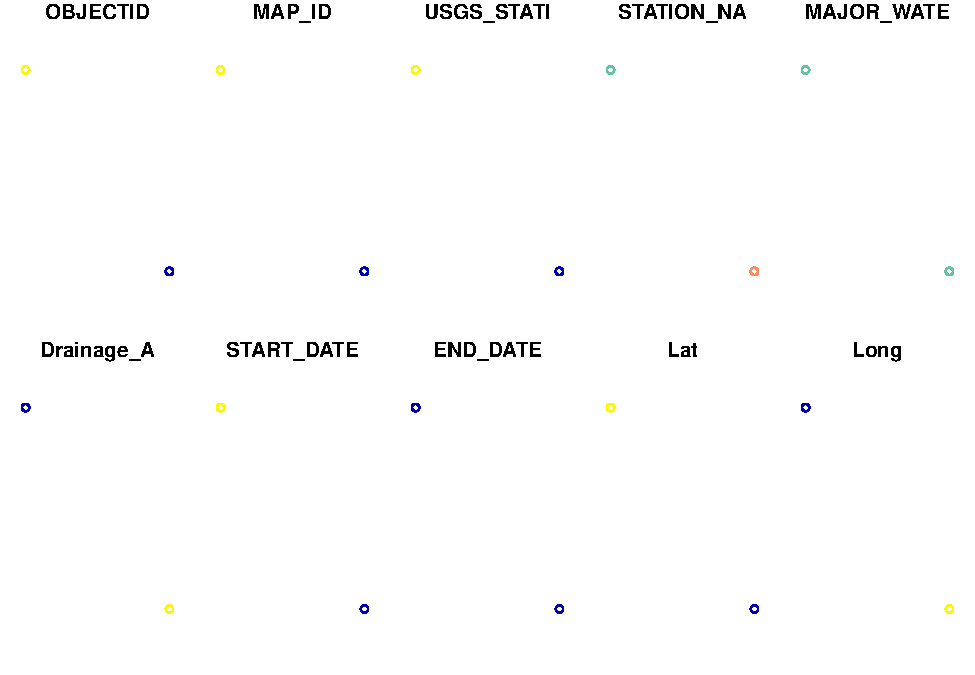
\includegraphics{lab01_files/figure-latex/mypoints-1.pdf} There are only
2 points, and the plot isn't super helpful without any other sort of
spatial reference, but you've succcessfully compelted your first spatial
operation in R!

\texttt{sf} has a number of other useful functions built-in that you can
try. For example, a quick calculation of the area of each county in
Delaware:

\begin{Shaded}
\begin{Highlighting}[]
\NormalTok{del.counties }\SpecialCharTok{\%\textgreater{}\%} \FunctionTok{st\_area}\NormalTok{() }
\end{Highlighting}
\end{Shaded}

\begin{verbatim}
## Units: [m^2]
## [1] 2065913885 3096294967 1278231147
\end{verbatim}

Note that \texttt{sf} gives you the units of the calculation, but also
that the data are in the form of a vector

\subsection{Your tasks}\label{your-tasks}

This lab requires you to put together many of the tasks demonstrated
above, in class, help documentation (don't forget the \texttt{?}
command!), and in your readings. I don't expect you'll know them all
immediately, so you'll need to reference those resources, your
classmates, and possibly web resources as well. This process is
representative of real-world problem solving in this domain. There are a
very large number of packages and functions available to you in R, and
no one person knows how to use them all. So be inventive, be clever, and
be persistent!

Complete each task COMPLETELY USING R CODE. YOU MUST SHOW YOUR WORK FOR
EACH ANSWER. Label your variables sensibly and use comments such that I
can find your answers and your work.

\subsubsection{Task 1: Basic data
manipulation}\label{task-1-basic-data-manipulation}

1.1 For each county, calculate its land area as percentage of the total
area (land + water) for that state.

1.2 For each state, find the county that has the largest proportion of
its land as water (water area / total area)

1.3 Count the number of counties in each state

1.4 Which station has the shortest name (STATION\_NA) in the study area?

\subsubsection{Task 2: Plotting attribute
data}\label{task-2-plotting-attribute-data}

\ldots for each plot, label your axes properly and give your plot a
title

2.1 Make a scatterplot showing the relationship between land area and
water area for each county. Color each point using the state variable

2.2 Make a histogram of drainage area (Drainage\_A) for all monitoring
stations

2.3 Make a similar histogram of drainage area (Drainage\_A) for all
monitoring stations. This time, shade/color each portion of the
histogram's bar(s) using the state variable

\subsubsection{Task 3: Write a function}\label{task-3-write-a-function}

3.1 Write a function that does the following:

A. accepts a vector of arbitrary numbers, calculates the mean, median,
maximum, and minimum of the vector

B. Sorts the vector

C. returns a list of those values from A and the sorted vector from B

D. the function should only work with numeric values and print an error
message if any other data type are found

Test it with the following vectors

\texttt{c(1,\ 0,\ -1),\ c(10,\ 100,\ 1000),\ c(.1,\ .001,\ 1e8),\ c("a",\ "b",\ "c")}

\subsubsection{Task 4: (slightly) more complex spatial
analysis.}\label{task-4-slightly-more-complex-spatial-analysis.}

\ldots Note, you may need to find supplementary data to help you with
these tasks

4.1 Calculate the number of monitoring stations in each state

4.2 Calculate the average size of counties in New York (that are also in
this study area)

4.3 Calculate which state has monitoring stations with the greatest
average drainage area (Drainage\_A)

\subsection{Questions}\label{questions}

\begin{enumerate}
\def\labelenumi{\arabic{enumi}.}
\tightlist
\item
  In using the intersection functions, are the following two statements
  equivalent? If not, explain how. Be sure to think about BOTH the
  spatial data structures AND the attribute data. Would your answer be
  different if we were using different types of data?
\end{enumerate}

\begin{verbatim}
 sf::st_intersection(d.stations, del.counties)
 sf::st_intersection(del.counties, d.stations)
\end{verbatim}

\begin{enumerate}
\def\labelenumi{\arabic{enumi}.}
\setcounter{enumi}{1}
\item
  What did you find challenging in this lab? What was new?
\item
  What types of activities would you like to see in labs this semester?
\end{enumerate}


\end{document}